\begin{document}

\chapter{Introduction}
\section{Research questions}

Due to its cross-platform capabilities, Progressive Web Apps seems like a promising alternative to native development. However, this shouldn't come at the cost of app performance and user experience, especially in regards to smoothness.
Thus, this paper will aim at answering the question : 
\begin{center}
    \textit{Can Progressive Web Apps be as smooth as Mobile Applications ?}
\end{center}
Which raises the following sub-questions: 
\begin{enumerate}
    \item What metrics are relevant to compare the smoothness of Mobile and Progressive Web Apps?
    \item What tools are available to measure those metrics ?
\end{enumerate}

\iffalse
Primary research question : 
\newline \textit{How efficient can Progressive Web Apps be compared to a Native Android Application?}
\newline
Secondary Research questions :
\\1. \textit{How can we compare Progressive Web Apps and Mobile Apps ?}
\newline \indent
1.1 \textit{What metrics are relevant to compare Progressive Web Apps and Mobile Apps ?}
\newline \indent  
1.2 \textit{What tools are available to measure those metrics?}
\newline
\\2. \textit{Are Progressive Web Apps more efficient than Mobile Apps with regards to the first question?}
\fi

Due to its cross-platform capability, Progressive Web Apps seems like a promising alternative to native development. However, this shouldn't come at the cost of app performance and user experience, especially in terms of the app smoothness and rendering capacity.
Thus, this paper will aim at answering the question : 
\begin{center}
    \textit{Are Progressive Web Apps more performant than Mobile Apps in terms of rendering capacity ?}
\end{center}
Which can be divided into the following sub-questions: 
\begin{enumerate}
    \item How can we compare Progressive Web Apps with Mobile Applications?
    \item What tools are available to measure the relevant metrics ?
\end{enumerate}

\chapter{Background}
\section{Mobile Applications}
\subsection{Development}

React Native, Ionic and PhoneGap are one of the most popular frameworks used today \cite{CrossPlatform_study}.

\section{Progressive Web Apps}
\subsection{Academic research}

Since June 2019, more than half of Web traffic comes from mobile devices. \cite{WebTrafficData}

    \cite{smoothnessQoE} build a model to evaluate the smoothness of smartphones. This model focuses on two major indexes : the maximum frame interval and the total number of frames in different key behavior scenarios (phone calls, browsing the web, playing games, etc). Those frames are defined as the interval of time between user input and response time of several key display events measured with a camera. %To check this frame definition
    
    \cite{PWAbc_responsetime} measured the response time between an Android app and a React PWA when accessing the Camera and Maps. The response time was measured 54 times for each scenario. The results show that Native are faster for accessing the camera, though PWAs are making progress in that regard. However, PWAs are faster regarding geolocation and map rendering.
    
    \cite{YbergViktor2018NPaU} focused on the user experienced of PWAs and measured several performance metrics: load times (Polymer, React, Preact), start-up times (native app, Polymer with and without browser in memory), Lighthouse performance audit (Polymer), list rendering times (PWA). He concluded that PWAs provided a good enough user experience for information access apps, though PWAs are not fully supported on every platform and web browser.
    
    \cite{PWApossibleUnifer}, followed by \cite{Biorn-Hansen2} shows a lack of academic research on the subject. \cite{PWApossibleUnifer} developped three apps using the Hybrid, Interpreted and PWA approach and compared their startup speed, app size and rendering speed. They conclude that PWA have a lot of potential to unify web and mobile development, though some limitations remains (lacking some hardware access, and browser support on some platform).
    
    \cite{Biorn-Hansen2} developed 5 apps: a PWA, a native app written in Kotlin, an Ionic hybrid app, an Interpreted React Native app and a cross-compiled Xamarin app. Again, they measure the app size, the activity launch time and the time from app icon to toolbar rendering. They reconfirmed the potential of PWAs to have an important part in futur Mobile development, depending on iOS support. They are extremely small compared to other apps, and render content fast. Although they lack some hardware access, they are also the only ones testable before install. 
    
    \cite{SW_and_energy} studied the energy impact of service workers on PWAs. Their results showed no significant energy impact from service workers. However, it also showed different energy consumption of each PWAs
    
    \cite{JohannsenFabian2018PWAa} studied how turning a regular web app into a PWA affects the code complexity in Angular. It concluded that the main increasing factor is the understanding of the new concepts behind the service workers, but automated PWA tooling can decrease it.
    
    \cite{Pride_Prejudice} identified several security threats regarding PWAs
    
    \cite{bac_pwa_comparison} found that PWAs had a slower performance than regular web apps (with lighthouse performance metrics)
    
    \cite{PWA_UX_comparison_study} conducted an analysis of user experience when interacting with a regular web app, a native Android app and a PWA. The 8 participants had an overall good user experience on every platform.
    
    \cite{bac_pwa_performance} studied loading performance (first paint, etc) of PWA in comparison to Apache Cordova app and native android. The results differ between phones %Conclusion noot very clear on this one
    
    \cite{emulating_native_w_crossplatform} compared features from a cross-platform app, a native Android app and a PWA. They were also compared in a qualitative and a qualitative user studies. No real difference was found between the applications. The React Native app performed a little better on the quantitative study, and the PWA performed a little better on the qualitative study.
    
    \cite{PWADatabase} compare performance of same app developed multiple times with different parameters (framework, service-worker, optimization, etc)
    
    \cite{PWAapplicability} compared the same app developed 4 times : a) as a native iOS, b) a native Android, c) a web app and d) a pwa in regards to First Paint and Energy consumption. Regarding the First Paint metric, the PWA performed better against the web app and the native Android app. The difference with iOS might be because of the incomplete support of PWA on iOS. As for energy consumption, PWA seemed to consume less energy, but the number of experiments was not enough to really confirm that.

\section{Profiling tools}

In order to answer the answer the research question, several metrics will be measured across a number of experiments. The most important one is information regarding the frames produced by the application
%, with a target rate of 60 frame per second \citationneeded \todo{Why?}
. Other metrics will be measured to assess the rendering capacity of the applications : the \%CPU usage of the application as well as the memory used by the GPU. This section covers the tools available to automatically collect the data needed as well as the tools chosen for this study.  


\subsection{Android}
However, this tool is not suited for automatic data collection as the results are only available in charts. Moreover, it can have a high overhead \cite{nanoscope} making the collected data less precise.

\paragraph{}
\textbf{Android Debug Bridge} \cite{adb} is a command-line tool used to communicate with an Android device (physical or emulator) from a computer. It can be used to list available devices (command \textit{devices}), forward requests (command \textit{forward} or execute commands on the device (command \textit{shell}). It will be widely used during this study. 

\paragraph{}
\textbf{Dumpsys} \cite{dumpsys} used with \textit{adb shell} provides information about the device's system services. A lot of different services (thus information) is available through this command-line tool, for example the network, the battery usage, input events, \red{etc}. The most interesting services for this study are: \todo{Rephrase} 
\begin{itemize}
    \item \textit{gfxinfo} which provides information regarding the animation such as jank rate (percentage of frames considered janky ie not meeting the 60fps threshold), total number of frames since recording, etc. It can be used with two options : \textit{framestats} which gives additional information about the frame timestamps, and \textit{reset} which reset the information recorded until now. This information is retrieved by Android framework during the application run-time.
    
    \item \textit{cpuinfo} gives the \%CPU usage of each process running during a given interval of time. The system computes this information from the proc/stat/ files (similar to the files of the same name found on Linux systems) and displays it as the percentage of CPU time used over the total CPU time available in one CPU core with a 0.1\% precision. The information is updated whenever the system needs it and  \todo[color=cyan!20]{Do I cite the source code for that ?} \todo{Yes:)} at least every 30min so the output is not always up-to-date.  
    
    \item \textit{meminfo} takes a snapshot of the memory allocation and outputs the data in details. The main field of interested displays by this command is the amount of memory used for graphics buffer queues. Coincidentally, it also checks the information contained by \textit{cpuinfo} is up-to-date. Thus, it is also used in the experiments to update \textit{cpuinfo}
\end{itemize}

\paragraph{}
\textbf{Top} comes from the Linux command-line of the same name, but with limited options. It displays the process activity in real-time (\%CPU, memory used and other). Its source of information is the same as dumpsys. However, the \%CPU displayed is the percentage of CPU time used over the total CPU time available in the device, with a 1\% precision. This makes it less accurate especially for processes that doesn't consume a lot of CPU. Thus, this command-line was discarded in favor of dumpsys.

\paragraph{}
\textbf{Systrace} \cite{systrace} records a device activity during a short period of time and outputs it in the form of an html file. The file can be viewed on Chrome Browser and displays a timeline of events for each threads running during the recording. The events displayed depends on the categories selected when starting the recording. This tool isn't suitable for automated experiments but can be really helpful to understand the cause of a bottleneck or, as it is the case in this study, understand how Android system works.

\paragraph{}
\textbf{Systrace} \cite{systrace} records a device activity during a short period of time and outputs it in the form of an html file. The file can be viewed on Chrome Browser and displays a timeline of events for each threads running during the recording. The events displayed depends on the categories selected when starting the recording. This tool isn't suitable for automated experiments but can be really helpful to understand the cause of a bottleneck or, as it is the case in this study, understand how Android system works.

\paragraph{}
\textbf{Monkeyrunner} \cite{monkeyrunner} is a tool used to interact with an Android device from a Python script. Aside from sending events and executing \textit{adb shell} commands, it can also take screenshots to test the app. This tool was used to automate the experiment and remove the variables introduced by human interaction from the experiments. 

\subsection{Chrome}

As Progressive Web Apps are after all web applications that runs on the browser, many of the tools available depends on the browser running the app. Thus, the tools presented here may only apply to apps running on Chrome.

\paragraph{}
\textbf{Chrome DevTools} is a set of developer tools available in the Chrome Browser in order to inspect a page on the browser (the network, the performance, the memory, the elements, etc). The main tool of interest here is the \textit{Performance} panel \cite{chrome_devtools_perf} which can record certain events during a period of time and display a lot of information from these events. Among the features of interest are : the display of the duration of a frame as well as the CPU time used to compute it, a CPU, an FPS and a memory chart in addition to a timeline of different events recorded.

\paragraph{}
\textbf{Lighthouse} \cite{lighthouse} is an automated  tool used to assess any web page's quality but mainly targeting Progressive Web Apps \cite{PWApossibleUnifer}. It is available from the \textit{Audits} panel on Chrome Devtools and can retrieve a large number of metrics from an automated recording. Those metrics are classified into five different groups: Performance, Accessibility, Best Practices, Search Engine Optomization (SEO) and Progressive Web Apps, and give an overall score from 0 to 100. It was often used in previous research on PWA \cite{}

\section{Rendering pipeline}

\subsection{Android}
Multiple Application Renderers can communicate with SurfaceFlinger at the same time.   When an application needs to display something on the screen, it pushes a 'surface' to a BufferQueue shared with SurfaceFlinger. Every once in a while, usually in synchronization with the screen refresh rate, SurfaceFlinger wakes up and look into the BufferQueues.

\subsection{Chrome}
However, some stages can be skipped depending on the change between two frames.

\section{Problem analysis}
In the light of the background described above, this sections provides additional motivation and limitations for the research questions. 
\paragraph{}
\textbf{Motivation} \newline

Previous research about Progressive Web Apps performance focused mainly on the performance at start-up (loading time, first paint) but none was found that studied the rendering performance during use. To my best knowledge, this research will be the first to do so.

\medskip
\textbf{Limitations} \newline
As stated above, Android applications and Web Applications on Chrome share two components of the display pipeline (SurfaceFlinger and the Hardware Composer) but differ greatly in the Application Renderer. Thus this research will focus on comparing the smoothness of Android applications and Progressive Web Apps in regards to this last component. 

Thus, this paper will analyze smoothness performance of the applications by looking at the average frame duration, as well as CPU and memory used to compare the resources used. 

\iffalse
However, at the time of writing no study was found that examined the rendering performance of Progressive Web Apps. While it is important for the user that the app launches quickly \cite{launch_time}, it is also important that the app remains smooth during the time of use. \newline
Thus, this paper will try to address this issue and study the smoothness of mobile applications and progressive web apps.

Most of the time, the smoothness of an application is associated with its responsiveness i.e. how quickly it can respond to user input.

As defined by nanana, "the principle of smoothness states that objects must change in a continuous fashion, which reduces cognitive load by removing large and unexpected changes in visual information presented to the user". In other words, a smooth animation changes frames and with little changes between them 

In this work, the smoothness of an application is defined as how quickly it can change the display

\paragraph{}
The smoothness of a mobile application is usually evaluated using the frame rate, or FPS for frame rate per second \cite{smoothnessQoE} \todo[inline]{It would be good to clarify what is smoothness and fluidness}. Though as Biørn-Hansen et al. pointed out while studying animation performance in mobile applications, the FPS metric does not give much insight about the fluidness of a user interface where animations run only during a short amount of time and the remaining time is spent idle waiting for new inputs.
\newline
Thus, this paper will analyze the smoothness performance of the applications by looking at the average frame duration, as well as CPU and memory used to compare the resources used. 
\fi

\chapter{Methodology}
\section{Comparing the Rendering Process}
   
    The background section presented an overview of Android's Garphics pipeline, with the Application Renderer itself divided into 7 stages : input handling, animation, measurement and layout, draw, sync and upload, issue commands, process and swap buffers. 
    
    It is possible to extract detailed information about an Android application frames thanks to the command \textit{adb shell dumpsys gfxinfo framestats}. This outputs multiple graphic information, such as total number of frames rendered, number of janky frames
    
    We can observe some of those stages in a Systrace recorded with the command: \textit{python systrace.py sched gfx view app -a [package-name] -o [output-file]}.
    
    \begin{figure}[!ht]
        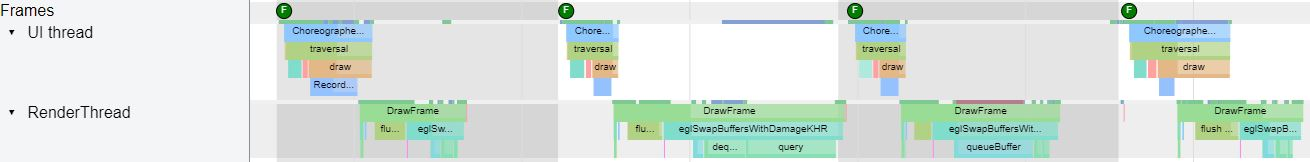
\includegraphics[width=15cm]{kththesis/Figures/android_systrace_frame.jpg}
        \caption{Application Renderer on Android}
        \label{fig:android_systrace}
    \end{figure}
    
    
    \subsection{Chrome's pipeline}
    \todo[inline, color=cyan!20]{Describe Chrome's pipeline model and how I came up with it}
       As was described in the Background chapter, Chrome contains several processes, including the Browser Process, the Renderer and the GPU Process.
    \subsection{Method of comparison}
    \todo[inline, color=cyan!20]{Conclusions on how to compare both pipelines: a) definition of a frame b) benchmark apps used}
\section{Comparing CPU and Memory}
    \subsection{Android and Chrome tools}
    \todo[inline, color=cyan!20]{Describe available tools on Android and Chrome}
    \todo[inline]{Move to Background}
    \subsection{Evaluating Chrome tools}
    \todo[inline, color=cyan!20]{Describe Experiments used to compare Android and Chrome tools, and their results}
    \subsection{Evaluating Emulators}
    \todo[inline, color=cyan!20]{Explain why Emulators are no good for evaluating CPU and Memory}

We will focus on the fluidity of the apps that can be defined with Frame Per Second (FPS) rate.
Thus, we will compare the FPS rate of a Native Android Application and a Progressive Web App, as well as with a benchmark consisting of : 
    - an app displaying different image/texts every 16/17ms
    - an app with more effort on the CPU : modification of the same pictures/texts or new pictures/texts generated randomly.
\newline

We will measure FPS, CPU and Memory usage to see the impact of CPU and Memory usage in the fluidity of the app.
\newline

\subsection{Scripts implementation}
\todo[inline]{Explain your technical contributions}

\end{document}